\section{Estado de avance}

Para comenzar el desarrollo de ChiVO fue necesario identificar aparte de los 
requerimientos y casos de uso, las interacciones que los usuarios iban a tener 
con el sistema. El diagrama de secuencia de interacción entre el usuario y el 
ChiVO se puede ver en la figura \textbf{referencia secuencia}. 
En base a este diagrama, requerimientos y tecnologías utilizadas el estado de 
avance se especificará por cada capa.

\begin{figure}[h]
    \centering
    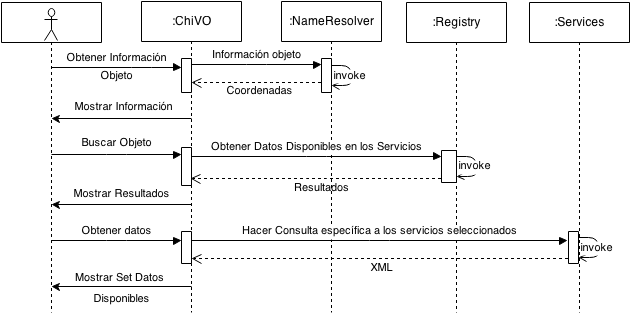
\includegraphics[width=0.45\textwidth]{images/secuencia.png}
    \caption{Diagrama de secuencia entre Usuario y ChiVO}
    \label{fig:secuencia}
\end{figure}

\textbf{Frontend}

Dento del diagrama de secuencia, el Frontend es el VO-Client, es decir, está a cargo de generar la interacción entre los usuarios y los demás elementos dentro del sistema.

Actualmente se generó un frontend en RoR que permite interactuar con: 
\begin{description}
 \item[Resolver nombres]:\hfill \\
  a partir de un nombre (String) retorna la posición de un objeto en coordenadas celestiales usando el servicio SESAME \textbf{TODO: ref} de Astrogrid.
 \item[Registro]: \hfill \\
 busca servicios dentro del endpoint, y luego según lo que necesite el usuario elige sobre cuales trabajar para hacer consultas. 
 \item[Servicios]: \hfill \\
 consulta a diferentes servicios web que proveen datos mediante cierto protocolo y unifica los resultados en un XML VOTable para ser desplegados en forma ordenada usando una biblioteca de javascript VOView.
\end{description}

\textbf{Endpoint}

El Endpoint está a cargo de generar una interacción transparente entre los clientes de VO y los posibles recursos que se configuren. En este caso el Endpoint genera una interfaz para los servicios configurados por el Backend y los disponibles a través del registro de VO-Paris. VO-Paris posee una Web API en REST que permite consultar por recursos y retorna un archivo JSON con resultados.

\textbf{Backend}

Actualmente ALMA le facilita a ChiVO datos públicos, los cuales incluyen ASDM, Measurement \cite{petry2012analysing}, FITS \cite{wells1981fits}, de los cuales es necesario extraer los metadatos del ObsCoreDM para ser ingresados a la base de datos.

\begin{figure}[h]
    \centering
    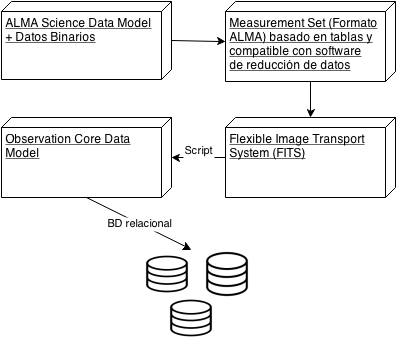
\includegraphics[width=0.45\textwidth]{images/metadata.png}
    \caption{Proceso transformación desde FrontEnd de ALMA hasta la base de datos de ChiVO}
    \label{fig:metadata}
\end{figure}

El procedimiento se hace a través de un script, el cual usando el framework de backend DaCHS \cite{dachs}, permite configurar recursos y servicios mediante archivos de configuración Resource Descriptor \cite{dachsorguide}. Una vez creadas las entradas en la base de datos y configurados los servicios SCS, SSAP, SIAP, TAP se pueden acceder mediante las consultas definidas en cada protocolo.




